% Sixty, Five, and Two: A Finite-Group Formalisation of Bazi
% Sukai <2396593357@qq.com>
% Compile: pdflatex main.tex  (run twice for references)

\documentclass[11pt,a4paper]{article}

\usepackage[margin=1in]{geometry}
\usepackage{amsmath,amssymb,amsthm,mathtools}
\usepackage{enumitem}
\usepackage{booktabs}
\usepackage{array}
\usepackage{tikz}
\usetikzlibrary{arrows.meta,calc}
\usepackage[super,sort&compress]{natbib}
\usepackage[colorlinks=true,allcolors=blue]{hyperref}
\usepackage{cleveref}

% --- theorem environments ---
\newtheorem{theorem}{Theorem}[section]
\newtheorem{proposition}[theorem]{Proposition}
\newtheorem{lemma}[theorem]{Lemma}
\newtheorem{corollary}[theorem]{Corollary}
\theoremstyle{definition}
\newtheorem{definition}[theorem]{Definition}
\theoremstyle{remark}
\newtheorem*{remark}{Remark}
\newtheorem*{note}{Note}

% --- shortcuts ---
\DeclareMathOperator{\lcm}{lcm}
\newcommand{\Z}{\mathbb{Z}}
\newcommand{\F}{\mathbb{F}}
\newcommand{\ord}{\operatorname{ord}}
\newcommand{\ke}{\mathsf{ke}}

\title{\textbf{Sixty, Five, and Two:\\ A Finite-Group Formalisation of Bazi}}
\author{Sukai\\ \texttt{2396593357@qq.com}}
\date{\today}

\begin{document}
\maketitle

\begin{abstract}
I show that the traditional Chinese calendrical and fate-calculation system known as \emph{bazi} (the ``four pillars'' or eight characters), together with its constituent devices---the ten heavenly stems and twelve earthly branches (\emph{ganzhi}), the five phases (\emph{wuxing}) with their generating and overcoming relations, and the hexagrams of the \emph{Yijing}---admits a clean translation into elementary finite algebra. The sixty-term sexagenary cycle is the cyclic group $\Z_{60}$, realised as an index-$2$ subgroup of $\Z_{10}\times\Z_{12}$; the five-phase generative/overcoming system is a single cyclic group $C_5$ in which \emph{overcoming equals the square of generating}; the trigrams and hexagrams are vector spaces over the field $\F_2$; and the relations used by the operator layer (clashes, combinations, three-harmonies, ten-gods) are involutions, coset partitions, and product maps. I give a fully formal casting map $\Phi$ from a birth time to a state in $\Z_{60}^4$, including a closed form for the day pillar, $(\mathrm{JDN}+49)\bmod 60$. A recurring meta-observation runs through the paper---\emph{skeleton versus decoration}: precisely those relations that can be written as group laws coincide with the parts of the tradition that are internally uncontroversial, whereas the externally-imposed lookup tables coincide with the parts long disputed between schools---and, over time, the latter ceded mainstream authority to the former. The formalisation is implemented as a pure-function library, verified by property tests encoding the theorems and by cross-validation against an independent calendar library on $300$ random dates. I am at pains to stress that formalising the \emph{logic} of bazi does not validate its \emph{empirical} predictions; it only makes them, for the first time, sharp enough to test.
\end{abstract}

\newpage
\section*{Preface: an honest framing}
For a body of lore to count as scientific, a minimal and widely accepted recipe is the three-step process: \emph{observe} a regularity, \emph{formalise} it in some language, and \emph{test} the predictions of that language. On this reading the worn question of whether a traditional divinatory practice ``is scientific'' dissolves into three independent questions, which may be answered separately.

This note is concerned with the middle step only, applied to one such practice. Practitioners of bazi had, over a millennium ago, already completed the first two steps in their own symbolic language---the stems, the branches, the phases. I do not invent their content; I re-formalise it in the language of modern algebra, and I discover that the translation is surprisingly faithful. Whether the third step succeeds---whether bazi predicts anything about people---is an empirical question this paper explicitly does \emph{not} answer. What I claim is that, after the translation, that question becomes well-posed for the first time: the logic is pinned down, the predictions are unambiguous, and the matter can be handed to statistics. This is the sense in which the work below is, I hope, useful regardless of one's prior belief in the subject.

\newpage
\tableofcontents

\newpage
\section{Introduction}

\subsection{The translation thesis}
The symbolic devices of Chinese fate-calculation were built to encode periodicities that their inventors had observed: the solar year, the apparent motion of Jupiter, the cycle of climates and seasons. Lacking modern mathematical notation, the inventors encoded these periodicities in a discrete, named vocabulary---ten stems, twelve branches, five phases, sixty paired terms. The central empirical observation of this paper is that this vocabulary is not arbitrary: it is a \emph{finite algebraic structure}, and a remarkably coherent one. The stems form a cyclic group; the branches another; their legal pairings a third; the phases a fourth; the hexagrams a vector space. The relations between these objects---``clash'', ``combine'', ``generate'', ``overcome''---are group-theoretic operations.

My task is translation, nothing more. I replace each named object by its algebraic counterpart, and each traditional rule by an algebraic statement, and I check that nothing is lost. The advantage is the usual one: algebra is precise, unambiguous, mechanically checkable, and free of the interpretive drift that afflicts a purely textual tradition. A recurring thesis, developed throughout and collected in \cref{sec:skeleton}, is that this precision cleanly separates a tradition's \emph{structural skeleton}---forced by the algebra---from its \emph{culturally overlaid decoration}.

\subsection{Contributions}
The paper delivers five formal results, each with a short proof, and one meta-observation.
\begin{enumerate}[leftmargin=*]
  \item \textbf{Sixty.} The sexagenary cycle of paired stems and branches is the cyclic group $\Z_{60}$, namely the index-$2$ subgroup $G=\{(a,b)\in\Z_{10}\times\Z_{12}:a\equiv b\pmod 2\}$; it is generated by $(1,1)$ and has order $\lcm(10,12)=60$ (\cref{thm:sexagenary}).
  \item \textbf{Five.} The five-phase system of generating (\emph{sheng}) and overcoming (\emph{ke}) is a single cyclic group $C_5$: defining $\sigma(x)=x+1$ on the phases $\Z_5$, we have \emph{overcoming $=$ generating squared}, $\ke=\sigma^2$ (\cref{thm:wuxing}). The five phases are not governed by two independent rules but by the powers of one cycle.
  \item \textbf{Two.} The \emph{Yijing} trigrams and hexagrams are the vector spaces $\F_2^3$ and $\F_2^6$; the classical ``changing'' operations (cuogua, zonggua, bian) are $\F_2$-affine involutions (\cref{prop:yijing}).
  \item \textbf{The casting map $\Phi$.} A bazi chart is a point of $\Z_{60}^4$. I give $\Phi$ from a birth time to such a point, including a closed form for the day pillar $(\mathrm{JDN}+49)\bmod 60$ (\cref{thm:daypillar}), and we show the two classical ``escape'' rules (wuhu-dun, wuzi-dun) are the same affine map $x\mapsto 2x$ on stem indices.
  \item \textbf{Operators.} The ten-god map factors through $\Z_5\times\Z_2$; the three branch relations clash/combine/harm are involutions of $\Z_{12}$ with sharp invariants; and the four ``three-harmonies'' are the cosets of $\langle 4\rangle\le\Z_{12}$, i.e.\ the quotient $\Z_{12}/\langle 4\rangle\cong\Z_4$ (\cref{thm:involutions,thm:threeharmony}).
\end{enumerate}
The meta-observation (\cref{sec:skeleton}) is that relations expressible as group laws are exactly the parts of the tradition that no school disputes, while the relations that \emph{cannot} be so expressed are exactly the long-contested ones---which have, over the centuries, ceded mainstream authority to the former. Formalisation thus cleanly separates a structural skeleton from a culturally overlaid decoration.

\subsection{Scope and boundary}
I formalise the \emph{logic} of bazi. I do not assert, test, or endorse any empirical claim of the form ``such-and-such a configuration entails such-and-such a personality''. Such claims live one layer above this paper, in the consumer, and are explicitly out of scope. The contribution is to make those claims, for the first time, unambiguous enough to be tested---an interface for falsifiability, not a verdict.

\subsection{Related prior art}
Leibniz famously recognised the sixty-four hexagrams as binary numerals~\cite{leibniz1703}. The calendrical structure of the stems and branches is documented in the standard sinological literature~\cite{smith2008,needham1959}, and authoritative algorithms for calendar conversions appear in~\cite{dershowitz}. To my knowledge no prior work restates the internal \emph{relations} of bazi (the operator layer of \cref{sec:operators}) as group-theoretic objects, nor isolates the ``skeleton versus decoration'' distinction of \cref{sec:skeleton}.

\section{Preliminaries and notation}\label{sec:prelim}

We write $\Z_n=\Z/n\Z$ for the additive group (and ring) of integers modulo $n$, and $\F_2$ for the field with two elements $\{0,1\}$, whose addition is exclusive-or. A group $\Z_n$ is \emph{cyclic} of order $n$; any element $g$ generates the subgroup $\langle g\rangle=\{0,g,2g,\dots\}$, whose size is the \emph{order} $\ord(g)$, the smallest $k>0$ with $kg\equiv 0$. For $g\in\Z_m\times\Z_n$ one has $\ord(g)=\lcm(m',n')$ where $m',n'$ are the component orders. A \emph{coset} of a subgroup $H\le G$ is a set $g+H$; the cosets partition $G$, and the quotient $G/H$ inherits a group structure when $H$ is normal (automatic in abelian groups). An \emph{involution} is a map equal to its own inverse. The group theory used below is standard~\cite{dummitfoote}.

\paragraph{Indexing convention.} We index all cyclic sets from $0$, so that arithmetic is clean: the heavenly stem \emph{jia} is $0$, the branch \emph{zi} is $0$, the phase \emph{mu} (wood) is $0$, and so on. Name tables are consulted only for display; the algebra sees integers. With this convention \emph{parity is yin-yang}: an object of even index is \emph{yang}, of odd index \emph{yin}. We write $\pi(x)=x\bmod 2\in\F_2$ for the parity (yin-yang) fibration.

\section{The stems and branches: Sixty}\label{sec:ganzhi}

\subsection{Stems and branches as cyclic groups}

\begin{definition}[stems, branches]
The \emph{heavenly stems} are the elements of $\Z_{10}$ and the \emph{earthly branches} the elements of $\Z_{12}$, with the name tables of \cref{tab:names}.
\end{definition}

\begin{table}[h]\centering
\caption{Stems ($\Z_{10}$), branches ($\Z_{12}$), phases ($\Z_5$), with the parity class (even $=$ yang).\label{tab:names}}
\small
\begin{tabular}{c|cccccccccccc}
stem index & 0 & 1 & 2 & 3 & 4 & 5 & 6 & 7 & 8 & 9 & & \\
name & jia & yi & bing & ding & wu & ji & geng & xin & ren & gui & & \\
phase & mu & mu & huo & huo & tu & tu & jin & jin & shui & shui & & \\ \midrule
branch index & 0 & 1 & 2 & 3 & 4 & 5 & 6 & 7 & 8 & 9 & 10 & 11 \\
name & zi & chou & yin & mao & chen & si & wu & wei & shen & you & xu & hai
\end{tabular}
\end{table}

The phases (wood, fire, earth, metal, water) are the set $\Z_5$; the table also records the surjection $\tau:\Z_{10}\to\Z_5$ assigning each stem its phase, $\tau(a)=\lfloor a/2\rfloor$, which is $2$-to-$1$.

\subsection{The sexagenary group}

A \emph{ganzhi pair} is a couple $(a,b)\in\Z_{10}\times\Z_{12}$. Of the $10\cdot 12=120$ conceivable pairs, tradition uses only sixty. The reason is algebraic.

\begin{definition}[sexagenary set]
The \emph{sexagenary set} is $G=\{(a,b)\in\Z_{10}\times\Z_{12}:a\equiv b\pmod 2\}$.
\end{definition}

That is, a stem and a branch pair only when they share the same parity---\emph{yang} stems with \emph{yang} branches, \emph{yin} with \emph{yin}. This is the traditional rule, now a congruence.

\begin{theorem}[sexagenary group]\label{thm:sexagenary}
$G$ is a subgroup of $\Z_{10}\times\Z_{12}$ of order $60$, and $G\cong\Z_{60}$. Concretely, $G=\langle(1,1)\rangle$ and $\ord\big((1,1)\big)=\lcm(10,12)=60$.
\end{theorem}
\begin{proof}
The map $\varphi:\Z_{10}\times\Z_{12}\to\Z_2$, $\varphi(a,b)=(a-b)\bmod 2$, is a homomorphism, and $G=\ker\varphi$; hence $G$ is a subgroup. Since $|\Z_{10}\times\Z_{12}|=120$ and $|\operatorname{im}\varphi|=2$, we get $|G|=120/2=60$.

Let $g=(1,1)$. The order of $g$ is the smallest $k>0$ with $k\equiv0\pmod{10}$ and $k\equiv0\pmod{12}$, namely $\lcm(10,12)=60$. Thus $\langle g\rangle$ has $60$ elements; as $\langle g\rangle\subseteq G$ and both have size $60$, they are equal. A group generated by one element is cyclic, so $G\cong\Z_{60}$.
\end{proof}

\begin{corollary}
The ``sixty-year cycle'' of the tradition is not an empirical fact deserving explanation: it is $\lcm(10,12)$. The heavens may have supplied the factors ten and twelve; their union, however, was always going to be sixty.
\end{corollary}

\begin{remark}[cosmological origin of $10$, $12$, $60$]
The two periods are not arbitrary. The ten stems descend from a decimal ``week'' of day-names attested on Shang oracle bones; the twelve branches are widely supposed to track the apparent twelve-year circuit of Jupiter (\emph{suixing}), whose sidereal period is in fact $\approx11.86$ years. The pairing rule $a\equiv b\pmod2$ then forces the combined period to $\lcm(10,12)=60$, the figure the tradition has always used. The cosmological reading---that stems encode a solar/decimal rhythm and branches a Jovian one---is, in this algebra, simply the assertion that two cyclic clocks of relatively-prime-half period are being run in phase.
\end{remark}

The identification $G\cong\Z_{60}$ is via $k\mapsto(k\bmod 10,\,k\bmod 12)$, so that the $k$-th term of the cycle (\emph{jiazi}$=0$, \dots, \emph{guihai}$=59$) is determined by a single integer.

\begin{figure}[h]\centering
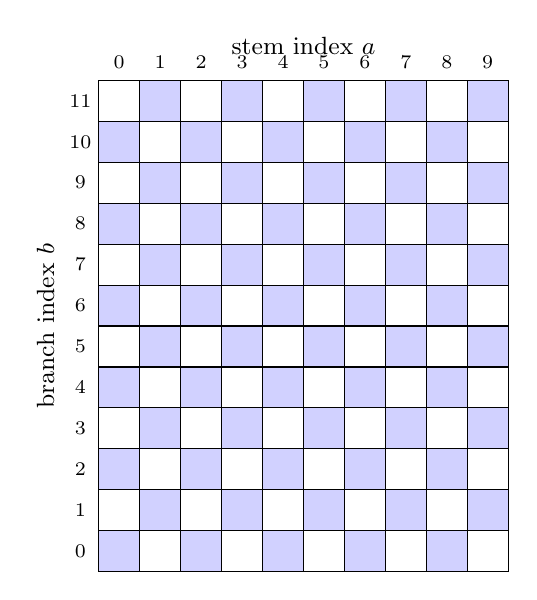
\begin{tikzpicture}[scale=0.52, every node/.style={font=\scriptsize}]
\foreach \i in {0,...,9}{\foreach \j in {0,...,11}{%
  \pgfmathtruncatemacro{\v}{mod(\i+\j,2)}%
  \ifnum\v=0 \fill[blue!18] (\i,\j) rectangle (\i+1,\j+1); \fi}}
\draw[thin] (0,0) grid (10,12);
\foreach \i in {0,...,9} \node at (\i+0.5,12.45) {\i};
\foreach \j in {0,...,11} \node at (-0.45,\j+0.5) {\j};
\node[above,font=\small] at (5,12.4) {stem index $a$};
\node[rotate=90,font=\small] at (-1.3,6) {branch index $b$};
\end{tikzpicture}
\caption{The $10\times12$ grid of conceivable ganzhi pairs; the $60$ shaded cells satisfy $a\equiv b\pmod 2$ and form the index-$2$ subgroup $G\cong\Z_{60}$ of \cref{thm:sexagenary}. The checkerboard makes the ``half of all pairs'' structure immediate.}\label{fig:grid}
\end{figure}

\subsection{The six decades and vacancy}
Tradition partitions the cycle into six \emph{xun} (decades) of ten consecutive terms, each opening with a stem \emph{jia}. The six opening indices form the subgroup $\langle 10\rangle=\{0,10,20,30,40,50\}\cong\Z_6$. Within the xun headed by $h$, ten stems are paired with only ten of the twelve branches, leaving two \emph{vacant}.

\begin{proposition}[vacancy, closed form]\label{prop:vacancy}
For a day index $k\in\Z_{60}$, taken as its canonical representative in $\{0,\dots,59\}$, with xun-head $h=k-(k\bmod 10)$, the two vacant branches are
\[
\mathrm{vac}(k)=\{(h-2)\bmod 12,\;(h-1)\bmod 12\}.
\]
\end{proposition}
\begin{proof}
The xun covers positions $h,h+1,\dots,h+9$, whose branches are $\{(h+i)\bmod 12:0\le i\le 9\}$---ten distinct residues of $\Z_{12}$. The two residues not covered are exactly $(h+10)\bmod 12$ and $(h+11)\bmod 12$, i.e.\ $(h-2)\bmod 12$ and $(h-1)\bmod 12$.
\end{proof}

\section{The five phases: Five}\label{sec:wuxing}

\subsection{Generating and overcoming}

The five phases $\Z_5=\{\text{mu},\text{huo},\text{tu},\text{jin},\text{shui}\}$ carry two fundamental relations, traditionally stated~\cite{hongfan} as independent rules:
\begin{itemize}[leftmargin=*]
\item \emph{generating} (\emph{sheng}): mu $\to$ huo $\to$ tu $\to$ jin $\to$ shui $\to$ mu;
\item \emph{overcoming} (\emph{ke}): mu $\to$ tu $\to$ shui $\to$ huo $\to$ jin $\to$ mu.
\end{itemize}

\begin{definition}
The generating map is $\sigma:\Z_5\to\Z_5$, $\sigma(x)=x+1$.
\end{definition}

\begin{theorem}[overcoming is generating squared]\label{thm:wuxing}
Define $\ke(x)$ as the phase overcome by $x$. Then $\ke=\sigma^2$. Hence the generating--overcoming system is the cyclic group $\langle\sigma\rangle\cong C_5\cong\Z_5$.
\end{theorem}
\begin{proof}
$\sigma^2(x)=x+2$. Reading the traditional overcoming list (mu $\to$ tu $\to$ shui $\to$ huo $\to$ jin $\to$ mu) off \cref{tab:names} gives the increments $2,2,2,2,2\pmod 5$; hence $\ke(x)=x+2=\sigma^2(x)$. As $\sigma$ is a $5$-cycle, $\langle\sigma\rangle=\{\mathrm{id},\sigma,\sigma^2,\sigma^3,\sigma^4\}$ has five elements and is cyclic of order $5$.
\end{proof}

\begin{remark}
This is the cleanest instance of the paper's thesis. A practitioner who memorised the generating and overcoming lists as two independent mnemonics has, without knowing it, memorised the \emph{same} cycle twice. Algebra is not correcting the tradition here; it is noticing that the tradition already knew. There is, structurally, only one rule.
\end{remark}

\begin{figure}[h]\centering
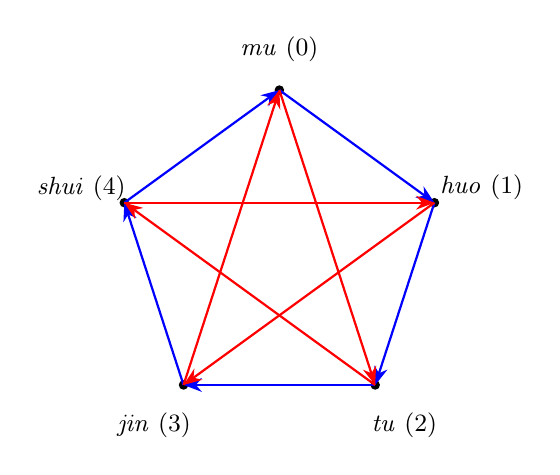
\begin{tikzpicture}[scale=1.15, >=Stealth, every node/.style={font=\small}]
\coordinate (mu)   at (90:1.8);
\coordinate (huo)  at (18:1.8);
\coordinate (tu)   at (-54:1.8);
\coordinate (jin)  at (-126:1.8);
\coordinate (shui) at (162:1.8);
\foreach \p in {mu,huo,tu,jin,shui} \fill (\p) circle (1.5pt);
\draw[blue,thick,->] (mu) -- (huo);
\draw[blue,thick,->] (huo) -- (tu);
\draw[blue,thick,->] (tu) -- (jin);
\draw[blue,thick,->] (jin) -- (shui);
\draw[blue,thick,->] (shui) -- (mu);
\draw[red,thick,->] (mu) -- (tu);
\draw[red,thick,->] (tu) -- (shui);
\draw[red,thick,->] (shui) -- (huo);
\draw[red,thick,->] (huo) -- (jin);
\draw[red,thick,->] (jin) -- (mu);
\node at (90:2.25)   {\emph{mu} (0)};
\node at (18:2.35)   {\emph{huo} (1)};
\node at (-54:2.35)  {\emph{tu} (2)};
\node at (-126:2.35) {\emph{jin} (3)};
\node at (162:2.3)   {\emph{shui} (4)};
\end{tikzpicture}
\caption{The five phases on a pentagon. Blue outer edges are the generating map $\sigma:x\mapsto x+1$; red inner chords are the overcoming map $\sigma^2:x\mapsto x+2$, tracing the inscribed pentagram. Overcoming is literally generating iterated twice (\cref{thm:wuxing}).}\label{fig:wuxing}
\end{figure}

\subsection{The relation matrix}

Any two phases $x,y$ stand in one of five relations, determined by their difference.

\begin{proposition}\label{prop:relmatrix}
The relation map $\mathrm{rel}(x,y)=(y-x)\bmod 5$ takes values in $\{0,1,2,3,4\}$ corresponding to \emph{same / I-generate / I-overcome / overcomes-me / generates-me}. Its matrix $M[x][y]=(y-x)\bmod 5$ is circulant, and off the diagonal satisfies $M[x][y]+M[y][x]\equiv0\pmod 5$.
\end{proposition}
\begin{proof}
$\mathrm{rel}$ depends only on $y-x$, so each row of $M$ is a cyclic shift of the previous: circulant. Moreover $M[y][x]=(x-y)\equiv-(y-x)\equiv -M[x][y]\pmod 5$, so the sum vanishes. This encodes the pairing ``I-generate / generates-me'' and ``I-overcome / overcomes-me'' as mutual inverses.
\end{proof}

\begin{table}[h]\centering
\caption{The circulant phase-relation matrix $M[x][y]=(y-x)\bmod 5$. Entries: $0=$same, $1=$I-generate, $2=$I-overcome, $3=$overcomes-me, $4=$generates-me.\label{tab:relmatrix}}
\small
\begin{tabular}{c|ccccc}
 & mu & huo & tu & jin & shui\\ \hline
mu  & 0 & 1 & 2 & 3 & 4\\
huo & 4 & 0 & 1 & 2 & 3\\
tu  & 3 & 4 & 0 & 1 & 2\\
jin & 2 & 3 & 4 & 0 & 1\\
shui& 1 & 2 & 3 & 4 & 0
\end{tabular}
\end{table}

\section{The Yijing: Two}\label{sec:yijing}

\subsection{Yin and yang as a field}
The two line types of the \emph{Yijing}~\cite{zhouyi} are the elements of $\F_2$: a \emph{yin} line is $0$, a \emph{yang} line is $1$. Addition in $\F_2$ is exclusive-or, which is precisely ``changing a line'' (yang becomes yin, yin becomes yang).

\begin{definition}
A \emph{trigram} is a vector of $\F_2^3$; a \emph{hexagram} is a vector of $\F_2^6$. We read a line of position $i$ (from the bottom) as bit $i$, so a hexagram is the integer $\sum_{i=0}^{5} b_i 2^i\in\{0,\dots,63\}$.
\end{definition}

There are $|\F_2^3|=2^3=8$ trigrams and $|\F_2^6|=2^6=64$ hexagrams---both numerically correct. The identification of the hexagrams with the binary numerals $0,\dots,63$ is exactly the observation Leibniz made three centuries ago~\cite{leibniz1703}.

\subsection{The changing operations are affine involutions}

\begin{proposition}[cuogua, zonggua, bian]\label{prop:yijing}
The classical ``changing'' operations on hexagrams are $\F_2$-affine maps and are involutions:
\begin{enumerate}[leftmargin=*]
  \item \emph{bian} (change line $i$): $b_i(x)=x\oplus 2^i$; translation by the unit vector $e_i$.
  \item \emph{cuogua} (invert all lines): $c(x)=x\oplus(2^6-1)=x\oplus 63$; translation by the all-ones vector.
  \item \emph{zonggua} (reverse the order of lines): $z(x)$, the bit-reversal of the six-bit representation; an $\F_2$-linear permutation.
\end{enumerate}
Each satisfies $f\circ f=\mathrm{id}$. Moreover $\F_2^6\cong\F_2^3\oplus\F_2^3$ splits a hexagram into its lower and upper trigrams.
\end{proposition}
\begin{proof}
Translations are affine; applying the same translation twice adds $2e_i=0$ in $\F_2$, giving the identity. Bit-reversal is a linear permutation of the six coordinate bits and is its own inverse. The splitting is the decomposition into the low three and high three bits.
\end{proof}

\begin{remark}[why the Yijing sits alongside bazi]\label{rem:najia}
Although the hexagrams are not wired into the four-pillar casting map, the two systems share both an origin (the stems--branches calendar) and, since the Han dynasty, an explicit bridge: the \emph{najia} (``incorporating the stems'') correlation assigns each trigram a set of heavenly stems and earthly branches, mapping the $\F_2^3$ of this section onto the $\Z_{10},\Z_{12}$ of \cref{sec:ganzhi}. The Yijing is included here as the third finite-algebraic system of the tradition, formally parallel to the other two, whether or not one adopts the najia bridge.
\end{remark}

\section{The bazi state space and the casting map \texorpdfstring{$\Phi$}{Phi}}\label{sec:bazi}

\subsection{State space}

A \emph{pillar} is an element of $G\cong\Z_{60}$ (\cref{thm:sexagenary}). A \emph{bazi chart} is a quadruple of pillars,
\[
\mathrm{chart}\;=\;(c_{\text{year}},c_{\text{month}},c_{\text{day}},c_{\text{hour}})\in G^4\cong\Z_{60}^4.
\]
The naive state space has $60^4\approx 1.3\times10^7$ points, but we shall see the four pillars are far from independent.

\subsection{Input and state; the casting map}
Let the \emph{input space} $\mathcal{I}$ be the continuous physical data (a birth instant, a longitude, a sex), and the \emph{state space} $\mathcal{S}=G^4$ (plus a derived sequence, the \emph{major cycles}). The \emph{casting map} is the quantising function
\[
\Phi:\mathcal{I}\longrightarrow\mathcal{S}.
\]
All the conventional controversy of bazi (where exactly does a year begin, how is the hour defined) lives inside $\Phi$; the algebra of $\mathcal{S}$ is uncontroversial. We decompose $\Phi$ pillar by pillar.

\subsubsection{Year pillar}
For a birth instant in Gregorian year $Y$, the year pillar is
\[
c_{\text{year}}=\big((Y-4)\bmod 10,\,(Y-4)\bmod 12\big),
\]
with the convention that the year increments at the solar term \emph{lichun} (early February). The constant $4$ is fixed by requiring the year $Y=4$ to be \emph{jiazi}; the parity constraint of \cref{thm:sexagenary} is then automatic.

\subsubsection{Month pillar: the wuhu-dun as an affine map}
Let $m_b\in\Z_{12}$ be the branch of the solar month containing the birth (determined by the solar terms), and let $a\in\Z_{10}$ be the year stem. The classical \emph{wuhu-dun} rule gives the month stem as
\[
c_{\text{month}}=\big(\,\big(2(a+1)+m_{\text{pos}}\big)\bmod 10,\;m_b\,\big),\qquad m_{\text{pos}}=(m_b-2)\bmod 12.
\]
A small but pleasing point: the map $a\mapsto 2(a+1)\bmod 10$ is \emph{affine in the year stem with coefficient $2$}; because $\gcd(2,10)=2$, its image is exactly the even (yang) stems. This is why, in the tradition, the opening month stem is always a yang stem---a fact usually memorised as a mnemonic and here seen to be a consequence of parity.

\subsubsection{Day pillar: a closed form}
The day pillar advances by one per day and never resets, independent of years and months.

\begin{theorem}[day pillar, closed form]\label{thm:daypillar}
For a Gregorian date $d$ with Julian Day Number $J(d)$, the bazi day index (\emph{jiazi}$=0$) is
\[
c_{\text{day}}=(J(d)+49)\bmod 60.
\]
\end{theorem}
\begin{proof}
The sexagenary day-count has run unbroken since the Shang oracle bones~\cite{needham1959}, so the day index advances by exactly one per day and has period $60$. This structural fact already reduces the problem to a single residue: for any reference date $d_0$ of known index $\iota_0$,
\[
\mathrm{index}(d)\equiv \iota_0+\big(J(d)-J(d_0)\big)\pmod{60}.
\]
The constant is therefore fixed by \emph{one} anchor alone. Taking $d_0=1949\text{-}10\text{-}01$, an attested \emph{jiazi} day ($\iota_0=0$) with $J(d_0)=2\,433\,191$, gives $c\equiv -J(d_0)\equiv 49\pmod{60}$, whence the formula. A second attested anchor---$1592$-$12$-$31$ is a \emph{jiashen} day (index $20$)~\cite{chenshu}---corroborates the value. (Before $1582$-$10$-$15$ the Julian calendar applies and the offset differs; this does not affect modern births.)
\end{proof}

\subsubsection{Hour pillar: the wuzi-dun}
With $h_b=\big\lfloor(\text{hour}+1)/2\big\rfloor\bmod 12$ giving the branch of the two-hour \emph{shichen} (for $\text{hour}\in\{0,\dots,23\}$), and $d\in\Z_{10}$ the day stem, the \emph{wuzi-dun} gives
\[
c_{\text{hour}}=\big(\,(2d+h_b)\bmod 10,\;h_b\,\big),
\]
again affine in the day stem with coefficient $2$, again with yang-stem image. Thus the two ``escape'' rules (wuhu-dun for months, wuzi-dun for hours) are the \emph{same} map $x\mapsto 2x$ on the relevant stem index, distinguished only by their offset.

\subsection{Reduced degrees of freedom}
\begin{proposition}\label{prop:dof}
The four pillars are not independent: $c_{\text{month}}$ is determined by $c_{\text{year}}$ and the solar term, and $c_{\text{hour}}$ by $c_{\text{day}}$ and the time of day. The genuine inputs are therefore $(Y,\text{term},\text{day-index},\text{shichen},\text{sex})$.
\end{proposition}

\subsection{The major cycles (dayun)}
From the month pillar one derives a sequence of pillars representing life epochs. Its direction is a parity computation.

\begin{proposition}\label{prop:dayun}
The major-cycle sequence runs forward (advancing in $\Z_{60}$) iff $\pi(\text{year stem})=\pi(\text{sex})$, where we encode male as $1$, female as $0$; otherwise it runs backward. The starting age is the number of days from the birth to the next (forward) or previous (backward) solar term, divided by three.
\end{proposition}

\section{The operator layer}\label{sec:operators}

The operator layer maps a chart to its ``annotations''---the relations the tradition reads off it~\cite{yuanhai}. I show these are algebraic.

\subsection{The ten gods factor through \texorpdfstring{$\Z_5\times\Z_2$}{Z5xZ2}}

\begin{proposition}[ten-god factorisation]\label{prop:tengod}
The \emph{ten-god} map $\mathrm{tg}:\Z_{10}\times\Z_{10}\to\{\text{10 classes}\}$ assigning to a day-master $a$ and another stem $b$ their relation factors as
\[
\mathrm{tg}(a,b)=F\big((\tau(b)-\tau(a))\bmod 5,\;\pi(a)=\pi(b)\big),
\]
where $\tau(a)=\lfloor a/2\rfloor$ and $\pi(a)=a\bmod 2$. In particular it depends only on the phase difference (five classes) and the parity match (two classes), yielding exactly $5\cdot 2=10$ gods.
\end{proposition}
\begin{proof}
Surjectivity: fixing $a=0$ and varying $b\in\Z_{10}$ yields the ten distinct gods of the classical table (\cref{tab:tengod}). The factorisation through $(\Z_5,\Z_2)$ is then immediate.
\end{proof}

\begin{table}[h]\centering
\caption{The ten gods as $(\text{phase-difference}\in\Z_5,\;\text{same parity?})$. ``Same'' is the \emph{pian} (indirect) column, ``different'' the \emph{zheng} (direct) column.\label{tab:tengod}}
\small
\begin{tabular}{c l l l}
\toprule
$d\in\Z_5$ & phase relation & same parity (\emph{pian}) & different parity (\emph{zheng})\\
\midrule
0 & same & bijian & jiecai\\
1 & I-generate & shishen & shangguan\\
2 & I-overcome & piancai & zhengcai\\
3 & overcomes-me & qisha & zhengguan\\
4 & generates-me & pianyin & zhengyin\\
\bottomrule
\end{tabular}
\end{table}

\subsection{Branch relations are involutions and a coset partition}

\begin{theorem}[clash, combine, harm are involutions]\label{thm:involutions}
The three branch relations are involutions of $\Z_{12}$:
\begin{itemize}[leftmargin=*]
  \item \emph{clash} (\emph{chong}): $\chi(b)=b+6$, with invariant $\chi(b)-b\equiv6$;
  \item \emph{combine} (\emph{he}): $\eta(b)=1-b$, with invariant $b+\eta(b)\equiv1$;
  \item \emph{harm} (\emph{hai}): $\rho(b)=7-b$, with invariant $b+\rho(b)\equiv7$.
\end{itemize}
Moreover $\chi$ is the unique non-trivial translation involution on $\Z_{12}$ (since $2d\equiv0\pmod{12}\iff d\in\{0,6\}$), and $\eta,\rho$ are reflections $b\mapsto c-b$.
\end{theorem}
\begin{proof}
Direct: $\chi(\chi(b))=b+12=b$; $\eta(\eta(b))=1-(1-b)=b$; $\rho(\rho(b))=7-(7-b)=b$. The invariants are read off the defining formulae.
\end{proof}

\begin{theorem}[three-harmonies are a coset partition]\label{thm:threeharmony}
The subgroup $\langle4\rangle=\{0,4,8\}\le\Z_{12}$ has order $3$, and its four cosets are exactly the four classical \emph{three-harmony} triples:
\[
\{0,4,8\},\;\{1,5,9\},\;\{2,6,10\},\;\{3,7,11\}.
\]
Hence the three-harmonies are the quotient $\Z_{12}/\langle4\rangle\cong\Z_4$, and membership of a branch $b$ is read off as $b\bmod 4$.
\end{theorem}
\begin{proof}
$\ord(4)=3$ since $3\cdot4=12\equiv0$ and no smaller multiple does. The cosets of a subgroup of order $3$ in a group of order $12$ are $12/3=4$ in number, each of size $3$, and are $r+\{0,4,8\}$ for $r=0,1,2,3$. These enumerate as stated, matching the traditional triples (shen-zi-chen, si-you-chou, yin-wu-xu, hai-mao-wei).
\end{proof}

\begin{figure}[h]\centering
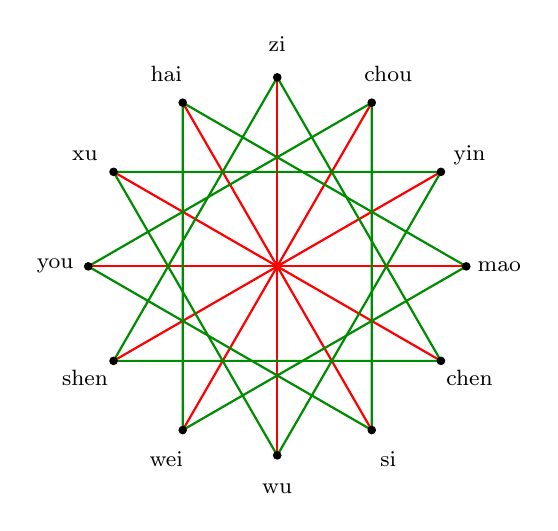
\begin{tikzpicture}[scale=1.2, every node/.style={font=\footnotesize}]
\def\R{2}
\foreach \i/\name in {0/zi,1/chou,2/yin,3/mao,4/chen,5/si,6/wu,7/wei,8/shen,9/you,10/xu,11/hai}{%
  \coordinate (b\i) at ({90-30*\i}:\R);
  \node at ({90-30*\i}:2.35) {\name};}
\foreach \i/\j in {0/6,1/7,2/8,3/9,4/10,5/11} \draw[red,thick] (b\i) -- (b\j);
\draw[green!55!black, thick] (b0) -- (b4) -- (b8) -- cycle;
\draw[green!55!black, thick] (b1) -- (b5) -- (b9) -- cycle;
\draw[green!55!black, thick] (b2) -- (b6) -- (b10) -- cycle;
\draw[green!55!black, thick] (b3) -- (b7) -- (b11) -- cycle;
\foreach \i in {0,...,11} \fill (b\i) circle (1.3pt);
\end{tikzpicture}
\caption{Branch relations on the $\Z_{12}$ circle. Red diameters are the clashes $b\leftrightarrow b{+}6$ (the unique non-trivial translation-involution, \cref{thm:involutions}); the four green equilateral triangles are the three-harmony cosets $\{r,r{+}4,r{+}8\}$, i.e.\ the four elements of $\Z_{12}/\langle4\rangle\cong\Z_4$ (\cref{thm:threeharmony}).}\label{fig:z12}
\end{figure}

\subsection{A consolidated table of branch relations}\label{sec:branchtable}
\Cref{tab:branchtable} records, for every branch, the partner forced by each of the five group-law relations (clash, combine, harm, three-harmony, three-direction); \cref{tab:branchlookup} records the two non-group relations (break, punishment). Read together they are a complete operator reference for $\Z_{12}$, and they make the dichotomy of \cref{sec:skeleton} tangible: the upper five relations are all generated by uniform formulae, the lower two by ad-hoc listings.

\begin{table}[h]\centering
\caption{Per-branch partners for the five group-law relations. Three-harmony gives the coset (with its synthesised phase); three-direction the consecutive triple (with the cardinal direction).\label{tab:branchtable}}
\resizebox{\textwidth}{!}{%
\begin{tabular}{c|c|c|c|c|c|c}
\toprule
idx & branch & clash ($b{+}6$) & combine ($1{-}b$) & harm ($7{-}b$) & three-harmony & three-direction\\
\midrule
0 & zi   & wu  & chou & wei & zi·chen·shen (shui) & hai·zi·chou (N)\\
1 & chou & wei & zi   & wu  & chou·si·you (jin)   & hai·zi·chou (N)\\
2 & yin  & shen& hai  & si  & yin·wu·xu (huo)     & yin·mao·chen (E)\\
3 & mao  & you & xu   & chen& mao·wei·hai (mu)    & yin·mao·chen (E)\\
4 & chen & xu  & you  & mao & zi·chen·shen (shui) & yin·mao·chen (E)\\
5 & si   & hai & shen & yin & chou·si·you (jin)   & si·wu·wei (S)\\
6 & wu   & zi  & wei  & chou& yin·wu·xu (huo)     & si·wu·wei (S)\\
7 & wei  & chou& wu   & zi  & mao·wei·hai (mu)    & si·wu·wei (S)\\
8 & shen & yin & si   & hai & zi·chen·shen (shui) & shen·you·xu (W)\\
9 & you  & mao & chen & xu  & chou·si·you (jin)   & shen·you·xu (W)\\
10& xu   & chen& mao  & you & yin·wu·xu (huo)     & shen·you·xu (W)\\
11& hai  & si  & yin  & shen& mao·wei·hai (mu)    & hai·zi·chou (N)\\
\bottomrule
\end{tabular}}
\end{table}

\begin{table}[h]\centering
\caption{The two non-group relations on $\Z_{12}$, recorded as listings.\label{tab:branchlookup}}
\small
\begin{tabular}{l|l}
\toprule
relation & members\\
\midrule
break (\emph{po}) & zi--you,\; chou--chen,\; yin--hai,\; mao--wu,\; si--shen,\; wei--xu\\
punishment (\emph{xing}) & yin$\to$si$\to$shen$\to$yin;\; chou$\to$xu$\to$wei$\to$chou;\; zi$\leftrightarrow$mao;\; self: chen, wu, you, hai\\
\bottomrule
\end{tabular}
\end{table}

\subsection{The luck pillars}
The vacancy of \cref{prop:vacancy} and the major cycles of \cref{prop:dayun} close the operator layer: both are group operations on $\Z_{60}$, computed from the day index and the month pillar respectively.

\subsection{Concrete lookups: the non-group operators}\label{sec:nonfit}
Three operator families resist expression as group laws, and I record them explicitly so that the contrast of \cref{sec:skeleton} is concrete.

\emph{Punishments} (\emph{xing}) form a directed graph on $\Z_{12}$ mixing three shapes: a directed triangle $2\to5\to8\to2$, another $1\to10\to7\to1$, a mutual pair $0\leftrightarrow3$, and four fixed points $4,6,9,11$. The step pattern within each triangle is $(+3,+3,+6)$, which is not a single group invariant. \emph{Breaks} (\emph{po}) are the six unordered pairs $\{0,9\},\{1,4\},\{2,11\},\{3,6\},\{5,8\},\{7,10\}$, all of constant difference $\pm3$ but with no uniform sign rule, so they do not arise as cosets. The \emph{nayin} assign one of the five phases to each of the sixty pairs via an external thirty-entry table (each entry serving two consecutive pairs); the phase sequence is not a residue of $k$ modulo any small integer and must be tabulated. None of the three is a homomorphism, an involution, or a coset partition.

\section{A birth, computed}\label{sec:example}
To make the casting map $\Phi$ concrete we apply it end to end. Consider a male birth at noon on $1984$-$02$-$15$.

\paragraph{Year pillar.} The birth is after \emph{lichun}, so $Y=1984$ and $c_{\text{year}}=((1984-4)\bmod10,(1984-4)\bmod12)=(0,0)$: \emph{jiazi}.

\paragraph{Month pillar.} The date lies in the solar month of branch \emph{yin} ($m_b=2$). With year stem $a=0$, the wuhu-dun gives month stem $2(0+1)+((2-2)\bmod12)=2$: \emph{bingyin}. Observe the opening stem is yang, as guaranteed by the coefficient $2$.

\paragraph{Day pillar.} From \cref{thm:daypillar}, $(\mathrm{JDN}(1984\text{-}02\text{-}15)+49)\bmod60=15$, i.e.\ $(5,3)$: \emph{jimao}.

\paragraph{Hour pillar.} Noon gives $h_b=\lfloor(12+1)/2\rfloor\bmod12=6$ (\emph{wu}). With day stem $d=5$, the wuzi-dun gives $(2\cdot5+6)\bmod10=6$: \emph{gengwu}.

The chart is therefore
\[
\text{\emph{jiazi}}\;/\;\text{\emph{bingyin}}\;/\;\text{\emph{jimao}}\;/\;\text{\emph{gengwu}}.
\]
The day master is \emph{ji} (yin earth). Two operators suffice to illustrate the layer. The \emph{ten-god} of the year stem \emph{jia} relative to the day master is, by \cref{prop:tengod}, $(\tau(0)-\tau(5))\bmod5=(0-2)\bmod5=3$ (``overcomes-me'') with differing parity (\emph{jia} yang, \emph{ji} yin), hence \emph{zhengguan} (direct officer). The \emph{vacancy} of the day index $15$ has xun-head $h=15-(15\bmod10)=10$, so by \cref{prop:vacancy} the vacant branches are $\{8,9\}$ (\emph{shen, you}).

Finally the major cycles (\cref{prop:dayun}) run forward, since the year stem \emph{jia} is yang and the native is male ($1=1$); the sequence opens from the month pillar \emph{bingyin} advancing by one, namely \emph{dingmao}, \emph{wuchen}, \emph{jisi}, \emph{gengwu}, \emph{xinwei}, $\dots$, beginning at age $6$. Every line of this example is the output of a group operation; none required consultation of a textual tradition.

\section{Skeleton versus decoration}\label{sec:skeleton}
Theorem after theorem of \cref{sec:operators} states that some traditional relation \emph{is} a group operation. \Cref{sec:nonfit} collects those that are not. The two lists are not arbitrary: they align with a sociological fact about the tradition.

\begin{table}[h]\centering
\caption{Skeleton versus decoration. The relations expressible as group laws are exactly those uncontested between schools; the rest are exactly the contested ones.\label{tab:skel}}
\small
\begin{tabular}{l l l}
\toprule
relation & algebraic status & controversy\\
\midrule
sexagenary cycle ($G\cong\Z_{60}$) & subgroup, cyclic generator & none\\
generating/overcoming ($C_5$) & powers of one cycle & none\\
clash / combine / harm & involutions & none\\
three-harmonies & cosets of $\langle4\rangle\cong\Z_4$ & none\\
three-directions & consecutive triples & none\\
ten-gods & factor through $\Z_5\times\Z_2$ & none\\
day pillar & closed form $(\mathrm{JDN}+49)\bmod60$ & none\\ \midrule
punishments (\emph{xing}) & directed graph (no group law) & disputed\\
breaks (\emph{po}) & six pairs (no group law) & disputed\\
nayin phases & external $30$-entry lookup & disputed\\
specific school's interpretations & empirical claims & intensely disputed\\
\bottomrule
\end{tabular}
\end{table}

We may read \cref{tab:skel} as follows, but the point is sharper than a static dichotomy. Read across time, it becomes a claim the tradition's own history bears out: over the centuries, the relations lacking algebraic enforcement \emph{ceded the mainstream} to those that possess it~\cite{smith1991,yuanhai,sanming}. The clearest case is \emph{nayin}---the core of the Tang-era \emph{luming} method (associated with Li Xuzhong)---which retreated into decoration while the later \emph{ziping} school, reading charts through the ten-gods and the orthodox stem-phases, hardened into the skeleton. What \emph{ziping} relies on is precisely the group-theoretic machinery above (the $C_5$ of the phases, the $\Z_5\times\Z_2$ of the ten-gods). And this is no coincidence: a relation forced by algebra is self-consistent, memorable, and checkable, so it survives oral and textual transmission intact; an arbitrary lookup has nothing to anchor it, and drifts between copyists and schools until it loses authority. Where a relation is forced by algebra, no school can coherently disagree, and indeed none does; where it is an external imposition, the tradition duly fragments. Structure, not taste, decided which parts of bazi would harden into canon and which would remain ornament.

This is, I believe, the most useful single contribution of the formalisation. It does not tell anyone whether to believe bazi, but it \emph{does} tell them precisely what they would be committing to: a minimal, uncontroversial, group-theoretic skeleton, plus a choice of decorative overlay. Disagreements that have spent centuries in the realm of textual exegesis can be relocated to their true home---the absence or presence of an underlying group law.

A second, methodological pay-off follows. Because the skeleton is now pinned to algebra, any \emph{empirical} claim of bazi (``this configuration yields that temperament'') can be stated unambiguously as a function of a chart, and handed to statistics. The decoration can be swapped, refined, or discarded without touching the skeleton. The formalisation is, in this sense, an interface for falsifiability. It is not lost on me that this paper itself observes the same discipline: its theorems are skeleton, its remarks decoration.

\section{Implementation}\label{sec:impl}
The formalisation is implemented as a pure-function library, \texttt{cbcm-core}, in roughly five hundred lines of Python. Each object of the paper---$\Z_{10},\Z_{12},\Z_{60},\Z_5,\F_2^3,\F_2^6$---is a module; each theorem is encoded as a property test that fails unless the theorem holds. Examples include $\ke=\sigma^2$ over all $x$, that clash/combine/harm are involutions, that the three-harmony cosets partition $\Z_{12}$, and that the ten-god map is exactly ten-valued.

Two observations from the implementation deserve record. First, the property tests are, in effect, a machine-checked version of the theorems: a bug in the algebra is a failed theorem. Second, the casting map $\Phi$ was end-to-end cross-validated against the independent library \texttt{lunar\_python} (v1.4, a widely used implementation of the traditional calendar) on $300$ birth dates drawn uniformly at random across the years $1960$--$2030$, comparing all four pillars in every case; all matched. The exercise caught two genuine errors during development, both instructive: the month stem was off by one cycle for the two ``pre-lichun'' months \emph{zi} and \emph{chou} (a missing $\bmod 12$ reduction of the month position), and the day pillar was advanced one day too early for births in the $23{:}00$ hour (the day should follow the civil calendar, with only the \emph{hour} stem borrowing the next day's stem at $23{:}00$). This is, I think, a small advertisement for the discipline of formalisation: the tests could not have been written without the algebra, and they located exactly the kind of boundary errors a tradition transmits orally and inconsistently.

The library and the scripts reproducing the cross-validation are publicly available.\footnote{\url{https://github.com/Shukahub/cbcm-Chinese-Birth-Chart-2-Math}}

\section{Conclusion}\label{sec:conclusion}
I have shown that the principal devices of Chinese fate-calculation---the stems and branches, the five phases, the hexagrams, the four pillars, and their operator relations---translate faithfully into elementary finite algebra: cyclic groups, a quotient group, a coset partition, a field-vector space, and a handful of affine maps and involutions. The translation is lossless in the sense that every traditional rule becomes a precise algebraic statement, and it is faithful in the sense that the relations so expressed are exactly the structural ones the tradition itself never disputes.

There is a final symmetry worth naming. To formalise a tradition is, in the end, to observe a regularity and invent names for it---which is precisely what the inventors of the stems and branches were doing three millennia ago. In this respect the algebraist and the diviner are not on opposite sides of the question; they are two readers of the same regularities, separated by notation and by a few thousand years of intermediate vocabulary. The paper does not so much replace the traditional language as recover, beneath it, the part that was always already mathematics.

I end where I began. Formalising the logic of bazi is not the same as validating its predictions. I have made no empirical claim and offer none. What the translation does provide is the precondition for any honest empirical inquiry: a fixed, unambiguous language in which the predictions of bazi can be stated, separated from the decorative overlays that obscure them, and---should anyone wish---tested. Whether the third step of the scientific recipe succeeds is a question for statistics, not for algebra. I merely hand over a language precise enough for the question to be asked.

\bigskip
\noindent\textbf{Acknowledgements.} The conceptual seed of this note is the observation that ``observe, formalise, test'' is a single recipe whose steps may be taken independently; the paper takes only the middle step.

\clearpage
\appendix

\section{The sixty ganzhi}\label{app:ganzhi}
The complete sexagenary cycle (\cref{thm:sexagenary}), indexed $k=0,\dots,59$ with \emph{jiazi}$=0$ and \emph{guihai}$=59$. Each entry is the pair $(k\bmod 10,\,k\bmod 12)$; parity is automatically matched.

\begin{center}\footnotesize
\resizebox{\textwidth}{!}{%
\begin{tabular}{|c|c|c|c|c|c|c|c|c|c|}
\hline
0 jiazi & 1 yichou & 2 bingyin & 3 dingmao & 4 wuchen & 5 jisi & 6 gengwu & 7 xinwei & 8 renshen & 9 guiyou\\ \hline
10 jiaxu & 11 yihai & 12 bingzi & 13 dingchou & 14 wuyin & 15 jimao & 16 gengchen & 17 xinsi & 18 renwu & 19 guiwei\\ \hline
20 jiashen & 21 yiyou & 22 bingxu & 23 dinghai & 24 wuzi & 25 jichou & 26 gengyin & 27 xinmao & 28 renchen & 29 guisi\\ \hline
30 jiawu & 31 yiwei & 32 bingshen & 33 dingyou & 34 wuxu & 35 jihai & 36 gengzi & 37 xinchou & 38 renyin & 39 guimao\\ \hline
40 jiachen & 41 yisi & 42 bingwu & 43 dingwei & 44 wushen & 45 jiyou & 46 gengxu & 47 xinhai & 48 renzi & 49 guichou\\ \hline
50 jiayin & 51 yimao & 52 bingchen & 53 dingsi & 54 wuwu & 55 jiwei & 56 gengshen & 57 xinyou & 58 renxu & 59 guihai\\ \hline
\end{tabular}}
\end{center}

The six rows correspond to the six \emph{xun} (decades) of \cref{prop:vacancy}; each opens with a stem \emph{jia}, and the six opening indices $\{0,10,20,30,40,50\}$ form the subgroup $\langle10\rangle\cong\Z_6$.

\section{The thirty nayin}\label{app:nayin}
The nayin assignment of \cref{sec:nonfit} in full. Each of the thirty entries serves two consecutive ganzhi (columns $k$); the right-hand column gives the synthesised phase. The phase sequence is not a residue of $k$ modulo any small integer, which is why the nayin resist a group-theoretic expression and must be tabulated.

\begin{center}\footnotesize
\begin{tabular}{c|l|c||c|l|c}
\hline
$k$ & nayin & phase & $k$ & nayin & phase\\ \hline
0--1   & haizhong-jin   & jin & 30--31 & sha-shi-jin    & jin\\
2--3   & luzhong-huo    & huo & 32--33 & shanxia-huo    & huo\\
4--5   & dalin-mu       & mu  & 34--35 & pingdi-mu      & mu\\
6--7   & lupang-tu      & tu  & 36--37 & bi-shang-tu    & tu\\
8--9   & jianfeng-jin   & jin & 38--39 & jinbo-jin      & jin\\
10--11 & shantou-huo    & huo & 40--41 & fu-deng-huo    & huo\\
12--13 & jianxia-shui   & shui& 42--43 & tianhe-shui    & shui\\
14--15 & chengtou-tu    & tu  & 44--45 & dayi-tu        & tu\\
16--17 & baila-jin      & jin & 46--47 & chaichuan-jin  & jin\\
18--19 & yangliu-mu     & mu  & 48--49 & sangzhe-mu     & mu\\
20--21 & quanzhong-shui & shui& 50--51 & daxi-shui      & shui\\
22--23 & wu-shang-tu    & tu  & 52--53 & sha-zhong-tu   & tu\\
24--25 & pili-huo       & huo & 54--55 & tian-shang-huo & huo\\
26--27 & songbai-mu     & mu  & 56--57 & shiliu-mu      & mu\\
28--29 & changliu-shui  & shui& 58--59 & da-hai-shui    & shui\\ \hline
\end{tabular}
\end{center}

\clearpage
\begin{thebibliography}{9}
\bibitem{leibniz1703} G.\,W.~Leibniz, ``Explication de l'arithm\'etique binaire,'' \emph{M\'emoires de l'Acad\'emie Royale des Sciences}, 1703.
\bibitem{hongfan} ``Hong Fan'' (``The Great Plan''), a chapter of the \emph{Shangshu} (\emph{Book of Documents}); the classical source for the five phases.
\bibitem{zhouyi} \emph{Zhouyi} (\emph{Book of Changes}); see in particular the \emph{Xici} (``Great Treatise'') appendix on the derivation of the trigrams and hexagrams.
\bibitem{smith2008} R.\,J.~Smith, \emph{Fathoming the Cosmos and Ordering the World: The Evolution of the Yijing and Its Readings}, University of Virginia Press, 2008.
\bibitem{needham1959} J.~Needham, \emph{Science and Civilisation in China}, vol.\ III, Cambridge University Press, 1959.
\bibitem{dershowitz} E.~Dershowitz and N.~Reingold, \emph{Calendrical Calculations}, Cambridge University Press (final edition).
\bibitem{smith1991} R.\,J.~Smith, \emph{Fortune-tellers and Philosophers: Divination in Traditional Chinese Society}, Westview Press, 1991.
\bibitem{yuanhai} \emph{Yuanhai Ziping} (``Profound Sea of Ziping''), Ming-dynasty compilation of the Song-dynasty \emph{ziping} corpus.
\bibitem{sanming} Wan Minying, \emph{Sanming Tonghui} (``Comprehensive Treatise on the Three Fates''), Ming dynasty; preserves the earlier \emph{luming} material.
\bibitem{chenshu} Chen Yuan, \emph{Ershishi Shuorun Biao} (Tables of the Months and Intercalations of the Twenty-Two Histories), 1926; reprinted, Zhonghua Bookshop. (The standard historical date index; consulted for the day-pillar anchors of \cref{thm:daypillar}.)
\bibitem{dummitfoote} D.~Dummit and R.~Foote, \emph{Abstract Algebra}, 3rd ed., Wiley, 2004. (For the standard group theory used throughout.)
\end{thebibliography}

\end{document}
